\section{計程車叫車問題 (Taxi)}

\subsection{問題描述}

你是某計程車公司老闆,擁有 \(m\) 台計程車。這些計程車都在 \(x\)
軸上,位置分別是 \(t_1, t_2, t_3, \ldots,t_m\)。同時,你接到 \(m\)
名路人的搭車請求,這 \(m\) 名路人也在 \(x\) 軸上,位置分別是
\(p_1, p_2, p_3, \ldots, p_m\)。我們假設上述 \(2m\)
個座標均相異。你的任務是為每一位路人指派一台計程車,且每台計程車只能指派給一位路人。你的目標是最小化這
\(m\)
台計程車到其指派路人的距離總和(稱此距離總和為叫車距離總和)。你的程式必須輸出最小叫車距離總和。

舉例來說,如果你有 \(2\) 台計程車(\(m=2\)),位置分別在 \(100\) 與
\(1\)(\(t_1=100, t_2=1\)),而 \(2\) 名路人位置分別在 \(3\) 與
\(101\)(\(p_1=3, p_2=101\)),則最小叫車距離總和為
\(|100-101|+|1-3|=3\)。

下圖顯示另一個例子。在這個例子中有\(5\)台計程車(\(m=5\)),位置分別在
\(3, 2, 1, 5, 4\)(\(t_1=3, t_2=2, t_3=1, t_4=5, t_5=4\)),而 \(5\)
名路人位置分別在
\(8, 6, 10, 9, 7\)(\(p_1=8, p_2=6, p_3=10, p_4=9, p_5=7\)),則最小叫車距離總和為
\(25\)(下圖所顯示的計程車指派方式之叫車距離總和即為 \(25\))。

\begin{center}
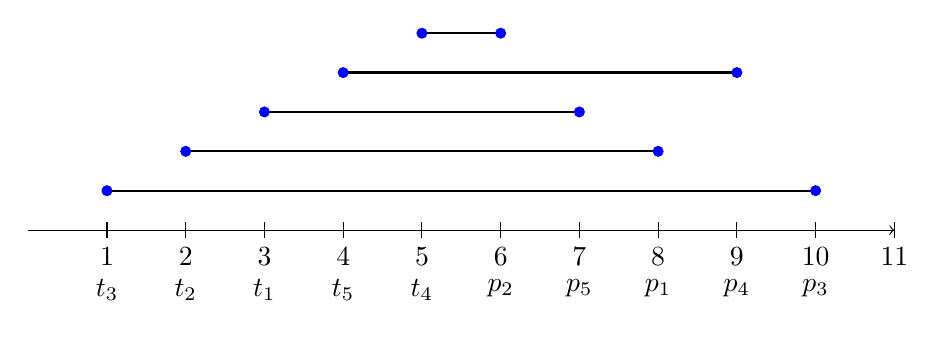
\begin{tikzpicture}
% Time axis
\draw[->] (0,0) -- (11,0) node[anchor=north west] {};
\foreach \x/\xtext in {1/1, 2/2, 3/3, 4/4, 5/5, 6/6, 7/7, 8/8, 9/9, 10/10, 11/11}
    \draw (\x,0.1) -- (\x,-0.1) node[anchor=north] {\xtext};

% Time labels
\foreach \x/\xlabel in {1/$t_3$, 2/$t_2$, 3/$t_1$, 4/$t_5$, 5/$t_4$, 6/$p_2$, 7/$p_5$, 8/$p_1$, 9/$p_4$, 10/$p_3$}
    \node[anchor=north] at (\x,-0.5) {\xlabel};

% Timelines
\draw[thick] (1,0.5) -- (10,0.5); % First line
\draw[thick] (2,1) -- (8,1);     % Second line
\draw[thick] (3,1.5) -- (7,1.5);% Third line
\draw[thick] (4,2) -- (9,2);     % Fourth line
\draw[thick] (5,2.5) -- (6,2.5);% Fifth line

% Points
\foreach \x/\y in {1/0.5, 10/0.5, 2/1, 8/1, 3/1.5, 7/1.5, 4/2, 9/2, 5/2.5, 6/2.5}
    \fill[blue] (\x,\y) circle (2pt);
\end{tikzpicture}
\end{center}

\subsection{輸入格式}

\begin{format}
\f{
$m$
$t_1$ $t_2$ $\ldots$ $t_m$
$p_1$ $p_2$ $\ldots$ $p_m$
}
\end{format}

\begin{itemize}
\tightlist
\item
  \(m\) 代表路人及計程車的數量。
\item
  \(t_i\)代表第\(i\)輛計程車的位置。
\item
  \(p_i\)代表第\(i\)個路人的位置。
\end{itemize}

\subsection{輸出格式}

\begin{format}
\f{
$a$
}
\end{format}

\begin{itemize}
\tightlist
\item
  \(a\) 代表給定輸入的最小叫車距離總和。
\end{itemize}

\subsection{測資限制}

\begin{itemize}
\tightlist
\item
  \(1 \leq m \leq 10^6\)。
\item
  \(1 \leq t_i \leq 2 \times 10^6\)。
\item
  \(1 \leq p_i \leq 2 \times 10^6\)。
\item
  保證給定的 \(2m\) 個座標均相異。
\end{itemize}

\subsection{範例測試}

\begin{example}
\exmp{
5
3 2 1 5 4
8 6 10 9 7
}{%
25
}%
\exmp{
5
10 70 30 90 50
71 31 51 91 11
}{%
5
}%
\end{example}

\subsection{評分說明}

本題共有兩組子任務,條件限制如下所示。
每一組可有一或多筆測試資料,該組所有測試資料皆需答對才會獲得該組分數。

\begin{longtable}[]{@{}ccl@{}}
\toprule
子任務 & 分數 & 額外輸入限制 \\
\midrule
\endhead
1 & \(40\) & \(\max_i\{t_i\} < \min_i\{p_i\}\)。 \\
2 & \(60\) & 無額外限制。 \\
\bottomrule
\end{longtable}

\section{分漆付款 (Paint)}

\subsection{問題描述}

兔子是「兔兔建設」的社長。最近公司的建設進度不如預期,經過兔子社長的調查後,發現原因出在負責運送油漆的粽子離職了!於是兔子社長決定雇用猩猩來完成原本粽子的工作。另外,在調查過程中兔子社長還發現,假如能在油漆搬運抵達之後將其進行分類,可以進一步提升裝潢部門的效率。於是兔子社長藉此機會,也將此任務安排給猩猩來完成。

根據規定,搬運完成的油漆桶會被擺放成一列。由於油漆桶非常重,猩猩每次只能將兩桶相鄰的油漆交換位置。兔子社長給猩猩的要求是將所有相同顏色的油漆桶擺在一起。舉例來說,假設油漆總共有
7 桶,其顏色分為紅綠藍三種,分別以 \texttt{R}、\texttt{G}、\texttt{B}
表示,而初始時此 7
桶油漆從左到右的排列為:\texttt{RRGGBGB},則猩猩只需要一次操作,便能把油漆桶排列為
\texttt{RRGGGBB}。又若初始時油漆桶的排列為:\texttt{GRRGBRB},則猩猩最少只要三次操作,便能把油漆桶排列為
\texttt{GGRRRBB}。

狡猾的兔子社長決定根據完成任務所需最少的交換次數來支付猩猩的薪水,假如給定油漆桶初始的排列,你能幫助猩猩算出最少的交換次數,來估計她應得的薪水嗎?

\subsection{輸入格式}

\begin{format}
\f{
$S$
}
\end{format}

\begin{itemize}
\tightlist
\item
  \(S\)
  為一個字串,代表油漆桶的排列順序,其中相同字符表示相同顏色的油漆桶,不同字符代表不同顏色。
\end{itemize}

\subsection{輸出格式}

\begin{format}
\f{
$m$
}
\end{format}

\begin{itemize}
\tightlist
\item
  \(m\) 代表最少的交換次數。
\end{itemize}

\subsection{測資限制}

\begin{itemize}
\tightlist
\item
  \(1 \le |S| \le {10}^{6}\)。
\item
  \(1 \le \textrm{distinct}(S) \le 7\)。
\item
  字串 \(S\) 由大小寫英文字母組成。
\item
  \(\textrm{distinct}(S)\) 代表字串 \(S\) 中字元種類的數量。
\end{itemize}

\subsection{範例測試}

\begin{example}
\exmp{
RRGGBGB
}{%
1
}%
\exmp{
GRRGBRB
}{%
3
}%
\exmp{
aAaaAaa
}{%
4
}%
\end{example}

\subsection{評分說明}

本題共有三組子任務,條件限制如下所示。
每一組可有一或多筆測試資料,該組所有測試資料皆需答對才會獲得該組分數。

\begin{longtable}[]{@{}ccl@{}}
\toprule
子任務 & 分數 & 額外輸入限制 \\
\midrule
\endhead
1 & \(21\) & \(\textrm{distinct}(S) \le 2\)。 \\
2 & \(26\) &
\(1 \le |S| \le {10}^{3}\),\(\textrm{distinct}(S) \le 3\)。 \\
3 & \(53\) & 無額外限制。 \\
\bottomrule
\end{longtable}

\section{數字叢集 (Nums)}

\subsection{問題描述}

小明暑假期間在某實驗室實習,主要工作就是協助實驗室整理大量的實驗數據。
實驗室累積了許多數據資料,但因設備及管理等問題,小明發現有些數據可能登記錯誤;
這些記錯的數字\textbf{恰好為原數字的兩個位數被互換}, 例如數字 \(1234\)
被記錄成 \(1324\) 或者數字 \(300\) 被記成 \(3\) 等等。

小明希望你寫出一個程式檢查哪些資料有可能被登記錯誤,具體來說他定義了一個關係函式
\(P(a, b)\), 若 \(a\) 將某兩個位數互換後與 \(b\) 相等,則
\(P(a, b) = \text{True}\);否則 \(P(a, b) = \text{False}\)。 舉例來說
\(P(3, 300) = \text{True}\), 因為 \(300\)
的第一位數和第三位數互換時會變成 \(3\); 但
\(P(1234, 2143) = \text{False}\),因為交換任何兩個位數都無法變成相同的數字。

小明想要將 \(n\) 個相異的非負整數 \(a_1, a_2, \cdots a_n\) 運用關係函式
\(P\) 來加以分群。 開始時,每一個數字可以自成一群, 對於一個數字 \(x\)
和一個群 \(S\), 如果 \(S\) 有一個成員 \(y\) 使得
\(P(x, y) = \text{True}\), 則將 \(x\) 所在的群與 \(S\)
合併,形成更大的群。

小明想知道這些數據可以分成幾群,群的個數越小越好,和最大的群有多少數字。請寫一個程式幫助小明完成此任務。

\subsection{輸入格式}

\begin{format}
\f{
$n$
$a_1 \ a_2 \ \ldots \ a_n$
}
\end{format}

\begin{itemize}
\tightlist
\item
  \(n\) 代表數字的個數。
\item
  \(a_i\) 代表第 \(i\) 個想分群的整數。
\end{itemize}

\subsection{輸出格式}

\begin{format}
\f{
$G_n$ \ $G_m$
}
\end{format}

\begin{itemize}
\tightlist
\item
  \(G_n\) 代表分群後群的個數。
\item
  \(G_m\) 代表分群後最大的群有幾個數字。
\end{itemize}

\subsection{測資限制}

\begin{itemize}
\tightlist
\item
  \(2 \le n \le 100\)。
\item
  \(a_i\) 的位數小於等於 \(5000\),\(n\)
  個數字皆相異且數字的前面不會有不必要的 \(0\) (leading zero)。
\item
  輸入的數皆為非負整數。
\end{itemize}

\subsection{範例測試}

\begin{example}
\exmp{
2
1234 1324
}{%
1 2
}%
\exmp{
6
1234 1324 2134 7 3 30
}{%
3 3
}%
\end{example}

\subsection{評分說明}

本題共有三組子任務,條件限制如下所示。
每一組可有一或多筆測試資料,該組所有測試資料皆需答對才會獲得該組分數。

\begin{longtable}[]{@{}ccl@{}}
\toprule
子任務 & 分數 & 額外輸入限制 \\
\midrule
\endhead
1 & \(15\) & \(n \le 20\) 且 \(a_i\) 的位數等於 \(5\)。 \\
2 & \(28\) & \(a_i\) 的位數小於等於 \(500\)。 \\
3 & \(57\) & 無額外限制。 \\
\bottomrule
\end{longtable}

\section{蓋蓋樂 (Cover)}

\textcolor{red}{\textbf{本題為 Output Only。}}請注意,你在第 \(i\)
筆測試資料上傳的輸出檔名必須為 \texttt{output\_i\_1.txt}。

\subsection{問題描述}

蓋蓋樂是一人策略遊戲。給定一個大棋盤,棋盤分成 \(m\times n\)
個區塊,相鄰區塊分別塗上白色與灰色以做區隔。每個區塊都是個 \(5\times 5\)
的方形小棋盤,每個小棋盤最多會有 \(2\)
個特殊的格子。舉例來說,下圖是一個 \(2\times 3\) 的大棋盤
\((m = 2, n = 3)\),其中有五個格子是特殊格子(以 \texttt{X} 標示)。

\begin{figure}[H]
\centering
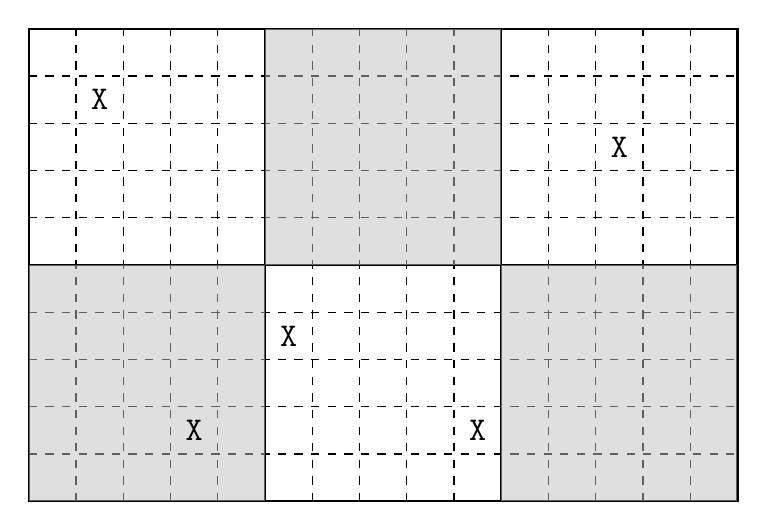
\begin{tikzpicture}[line width=0.4pt, scale=0.6]

% Define grid dimensions
\def\n{10} % Number of rows
\def\m{15} % Number of columns

% Draw the grid
\draw[dashed] (0, 0) grid (\m, \n);

% Add 5x5 bounding boxes
\foreach \x in {0, 5, 10} {
    \foreach \y in {0, 5} {
        \draw[thick] (\x, \y) rectangle (\x+5, \y+5);
    }
}

% Define shaded regions
\foreach \x in {1, 2, 3, 4, 5, 11, 12, 13, 14, 15} {
    \foreach \y in {1, 2, 3, 4, 5} {
        \fill[gray!50, opacity=0.5] (\x-1, \y-1) rectangle (\x, \y);
    }
}

\foreach \x in {6, 7, 8, 9, 10} {
    \foreach \y in {6, 7, 8, 9, 10} {
        \fill[gray!50, opacity=0.5] (\x-1, \y-1) rectangle (\x, \y);
    }
}

% Add X marks
\node at (1.5, 8.5) {\large \texttt{X}};
\node at (3.5, 1.5) {\large \texttt{X}};
\node at (12.5, 7.5) {\large \texttt{X}};
\node at (5.5, 3.5) {\large \texttt{X}};
\node at (9.5, 1.5) {\large \texttt{X}};

\end{tikzpicture}
\end{figure}

蓋蓋樂有兩種積木(如下圖所示),分別可用以蓋住棋盤上 \(4\) 或 \(3\)
個格子。兩種積木分別可以任意旋轉 \(0, 90, 180, 270\)
度後再蓋住棋盤格子,但是特殊的格子不可以被蓋住。

\begin{figure}[H]
\centering
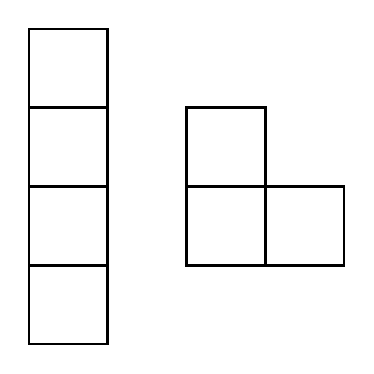
\begin{tikzpicture}[line width=1pt]

% Left stack of squares
\foreach \y in {0, 1, 2, 3} {
    \draw (0, \y) rectangle (1, \y + 1);
}

% Right L-shaped figure
\foreach \x/\y in {2/2, 2/1, 3/1} {
    \draw (\x, \y) rectangle (\x + 1, \y + 1);
}

\end{tikzpicture}
\end{figure}

請用以上兩種積木把大棋盤蓋滿(特殊格子除外),使得\textbf{共用積木的區塊對}越少越好。

\begin{itemize}
\tightlist
\item
  也就是說,只要有兩個區塊共用了同一塊積木,無論他們共用了幾塊,都會被算做一個「共用積木的區塊對」。你的目標就是最小化這個區塊對的數量。
\end{itemize}

在本題中,保證任意兩個特殊格子\textbf{皆不八方位相鄰}。也就是說,對於任兩個特殊格子座標
\((a, b), (c, d)\),皆有 \(\max(|a - c|, |b - d|) > 1\)。

\subsection{輸入格式}

\begin{format}
\f{
$n$ $m$
$a_{1, 1}$ $a_{1, 2}$ $\cdots$ $a_{1, 5m}$
$a_{2, 1}$ $a_{2, 2}$ $\cdots$ $a_{2, 5m}$
$\vdots$
$a_{5n, 1}$ $a_{5n, 2}$ $\cdots$ $a_{5n, 5m}$
}
\end{format}

\begin{itemize}
\tightlist
\item
  \(n, m\) 為棋盤的大小。
\item
  \(a_{i, j}\) 代表棋盤第 \(i\) 列第 \(j\)
  欄的格子是否為特殊格子(也就是不能被蓋住的格子),以 \(0\) 或 \(-1\)
  表示,其中 \(0\) 代表可被蓋住的棋盤格子,\(-1\) 代表特殊的格子。
\end{itemize}

\subsection{輸出格式}

\begin{format}
\f{
$b_{1, 1}$ $b_{1, 2}$ $\cdots$ $b_{1, 5m}$
$b_{2, 1}$ $b_{2, 2}$ $\cdots$ $b_{2, 5m}$
$\vdots$
$b_{5n, 1}$ $b_{5n, 2}$ $\cdots$ $b_{5n, 5m}$
}
\end{format}

請將棋盤蓋滿(特殊格子除外)後送回評分。積木蓋住棋盤的表示方式如下:

\begin{itemize}
\tightlist
\item
  同一塊積木需以相同的\textbf{正整數}作為代號,例如
  \(1, 2, 3, \ldots\),但代號最大不可超過 \(15000\)。特殊格子必須維持以
  \(-1\) 代表之。
\item
  不同塊積木\textbf{不可以}使用相同的代號。
\end{itemize}

\subsection{測資限制}

\begin{itemize}
\tightlist
\item
  \(1\le n\times m\le 1600\)。
\item
  \(-1 \leq a_{i, j} \leq 0\)。
\item
  輸入的數字皆為整數。
\item
  保證任一個被劃分出來的 \(5\times 5\)
  方形小棋盤內,特殊格子數量都不超過 \(2\)。
\item
  保證存在一種可以蓋滿棋盤的方式。
\item
  保證任意兩個特殊格子皆不八方位相鄰。
\end{itemize}

\subsection{評分說明}

本題共有 10 組測試資料,輸入檔案的說明如表所示。
對於每一組測試資料,若你上傳的輸出檔案滿足輸出格式,並且成功蓋滿了所有除了特殊格子以外的格子,那麼你會得到以下分數
\[
S \cdot \max\left(\frac{1}{10}, \frac{1}{\sqrt{q - p + 1}}\right) 
\] 其中 \(S\) 是該測試資料的分數比重,\(p\)
是最佳解的共用積木區塊對數量、\(q\)
是你給出的構造內的共用積木區塊對數量。

若你上傳的輸出檔案不滿足輸出格式、或是沒有蓋滿所有除了特殊格子以外的格子,那麼你將得到
\(0\) 分。

\begin{longtable}[]{@{}ccccl@{}}
\toprule
測試資料 & 分數比重 \(S\) & 輸入檔名 & 輸出檔名 & 說明 \\
\midrule
\endhead
1 & \(4\) & \texttt{input\_1\_1.txt} & \texttt{output\_1\_1.txt} &
\(n = 1\),\(m = 1\)。 \\
2 & \(4\) & \texttt{input\_2\_1.txt} & \texttt{output\_2\_1.txt} &
\(n = 1\),\(m = 2\)。 \\
3 & \(6\) & \texttt{input\_3\_1.txt} & \texttt{output\_3\_1.txt} &
\(n = 1\),\(m = 3\)。 \\
4 & \(8\) & \texttt{input\_4\_1.txt} & \texttt{output\_4\_1.txt} &
\(n = 2\),\(m = 2\)。 \\
5 & \(10\) & \texttt{input\_5\_1.txt} & \texttt{output\_5\_1.txt} &
\(n = 10\),\(m = 10\)。 \\
6 & \(12\) & \texttt{input\_6\_1.txt} & \texttt{output\_6\_1.txt} &
\(n = 10\),\(m = 10\)。 \\
7 & \(8\) & \texttt{input\_7\_1.txt} & \texttt{output\_7\_1.txt} &
\(n = 1\),\(m = 1599\)。 \\
8 & \(20\) & \texttt{input\_8\_1.txt} & \texttt{output\_8\_1.txt} &
\(n = 20\),\(m = 24\)。 \\
9 & \(20\) & \texttt{input\_9\_1.txt} & \texttt{output\_9\_1.txt} &
\(n = 40\),\(m = 40\)。 \\
10 & \(8\) & \texttt{input\_10\_1.txt} & \texttt{output\_10\_1.txt} &
\(n = 39\),\(m = 39\)。 \\
\bottomrule
\end{longtable}

\newpage

\subsection{範例}

作為範例,假設測試資料的長相為

\begin{verbatim}
2 3
0 0 0 0 0 0 0 0 0 0 0 0 0 0 0
0 -1 0 0 0 0 0 0 0 0 0 0 0 0 0
0 0 0 0 0 0 0 0 0 0 0 0 -1 0 0
0 0 0 0 0 0 0 0 0 0 0 0 0 0 0
0 0 0 0 0 0 0 0 0 0 0 0 0 0 0
0 0 0 0 0 0 0 0 0 0 0 0 0 0 0
0 0 0 0 0 -1 0 0 0 0 0 0 0 0 0
0 0 0 0 0 0 0 0 0 0 0 0 0 0 0
0 0 0 -1 0 0 0 0 0 -1 0 0 0 0 0
0 0 0 0 0 0 0 0 0 0 0 0 0 0 0
\end{verbatim}

則下面是一個可能的合法輸出

\begin{verbatim}
1 1 2 2 3 3 11 12 12 12 12 21 21 21 21
1 -1 2 4 3 13 11 11 14 15 15 15 15 22 22
5 5 6 4 4 13 13 16 14 14 23 23 -1 22 24
5 7 6 6 8 8 17 16 16 18 23 25 25 24 24
9 7 7 10 8 19 17 17 20 18 18 25 26 27 27
9 9 28 10 10 19 19 35 20 20 41 26 26 27 42
29 29 28 28 30 -1 36 35 35 37 41 41 43 42 42
29 31 32 32 30 30 36 36 38 37 37 43 43 44 44
31 31 32 -1 33 33 39 38 38 -1 45 45 45 45 44
34 34 34 34 33 39 39 40 40 40 40 46 46 46 46
\end{verbatim}

在這個範例中,最佳解的共用積木區塊對數量為
\(1\),而上面輸出的任兩個相鄰區塊都有共用積木,得到區塊對數量為
\(7\),表示 \(p\) 和 \(q\) 的值分別為 \(1\) 和 \(7\)。因此,假設分數比重
\(S=10\),這個輸出可以獲得
\(S\cdot\max\left(\frac{1}{10}, \frac{1}{\sqrt{7 - 1 + 1}}\right) \approx 3.78\)
分。

\subsection{視覺化工具(Visualizer)}

為了方便選手觀看自己的輸出結果以及觀察測試資料,在此任務的附件(attachment)中,有一腳本程式(script)供選手視覺化(visualize)輸入檔與輸出檔。

請利用下列指令視覺化輸入檔。

\begin{verbatim}
python3 visualizer.py [input file]
\end{verbatim}

你可利用下列指令,將你對於某個輸入計算出的解做視覺化。因為技術上的限制,附件中提供的視覺化工具在棋盤過大時,僅會顯示前
\(10\) 排、以及前 \(10\) 欄的方形小棋盤。

\begin{verbatim}
python3 visualizer.py [input file] --solution [output file]
\end{verbatim}

為了方便辨識,程式會以上色每塊積木的方式輸出,而不輸出積木上面的數字。但由於顏色數量有限,程式會重新為所有積木上色並僅保證相鄰的積木不同色。

範例:

\begin{verbatim}
python3 visualizer.py input_1_1.txt --solution output_1_1.txt
\end{verbatim}

請注意,若你傳入的資料的格式並不合法,將會產生一些不可預期的行為。不過,當你的解答唯一違反的規則是「未蓋滿所有格子」時,將未被蓋到的格子留下數字
\(0\) 會讓該格子呈現白色,並正常的進行視覺化。

一張使用前面範例所提到的視覺化成果圖如下:

\begin{figure}[!htb]
  \centering
  \includegraphics[width=0.5\linewidth]{cover.png}
\end{figure}

\section{花果山 (Huaguo)}

\subsection{問題描述}

在遙遠的花果山上,這裡景色壯麗,四季如春,瀑布飛流直下,桃樹繁茂,彷彿一片世外桃源。這裡的居民是一群聰明靈活的猴子,牠們以這片山林為家,過著看似自由而快樂的生活。然而,隨著時間的推移,猴群之間逐漸出現了貧富不均的問題。部分猴子佔據了最好的桃樹,享受著山上最豐富的資源,而其餘的猴子則只能在乾涸的山坡上勉強糊口。

這種不公平的現象日益嚴重,猴子們的怨言也隨之增加。富有的猴子漸漸習慣了掌握資源和地位,漠視了其他猴子的困苦。而那些身處底層的猴子,每天都在為食物而爭奪,生活艱難。這樣的社會狀況讓整個花果山逐漸陷入了混亂與不滿之中。

「我們不能再這樣下去了!」花果山的統治者猴王孫悟空在一次花果山政府會議上說道。「我們必須立刻改變!從現在起,花果山所有桃樹結下的桃子,由政府直接接收後,再重新分配給花果山上的猴子,直到所有猴子都擁有等量的桃子為止!」

孫悟空要求花果山政府統計所有猴子所擁有的桃子以及桃樹每天的桃子產量。花果山統計局很快地將相關數據呈給孫悟空:花果山上總共有
\(n\) 隻猴子,第 \(i\) 隻猴子擁有 \(a_i\)
顆桃子,而桃樹的產量很穩定,每天都能夠生產出 \(k\) 顆桃子。

花果山的內政大臣天命人針對重新分配的方法,向孫悟空提出建言:「為了花果山上的和諧,重新分配桃子時,政府不可以從猴子手中奪走任何桃子。政府每天接收到的桃子,必須當天就分配出去。最重要的是要避免相對剝奪感,每一天分配到最多桃子的猴子,只能比分配到最少桃子的猴子多得一顆桃子。」孫悟空覺得很有道理,便要求按照天命人的建議進行分配。

假設 \(n=4,k=7,a_1=1,a_2=2,a_3=3,a_4=4\),即花果山上總共有 4
隻猴子,分別有 1, 2, 3, 4 顆桃子,而桃樹每天的產量是 7
顆桃子。按照天命人的建議,每隻猴子每天都可以分配到一顆或是兩顆桃子,不能更少也不能更多,否則會帶來相對剝奪感。此時可以透過下列步驟,讓所有的猴子擁有等量的桃子:

\begin{enumerate}
\def\labelenumi{\arabic{enumi}.}
\tightlist
\item
  第一天到第三天都分配各兩顆桃子給前三隻猴子、一顆桃子給第四隻猴子。三天過後,四隻猴子分別擁有
  7, 8, 9, 7 顆桃子。
\item
  第四天、第五天都分配各兩顆桃子給前兩隻猴子、一顆桃子給第三隻猴子、兩顆桃子給第四隻猴子。五天過後,四隻猴子分別擁有
  11, 12, 11, 11 顆桃子。
\item
  第六天分配一顆桃子給第二隻猴子、各兩顆桃子給其餘的三隻猴子。六天過後,四隻猴子分別擁有
  13, 13, 13, 13 顆桃子,數量相等。
\end{enumerate}

請撰寫一個程式計算,最少要幾天之後,才能使得所有的猴子都擁有等量的桃子。

\subsection{輸入格式}

輸入包含多筆測試資料

\begin{format}
\f{
$T$
$\text{testcase}_1$
$\text{testcase}_2$
$\vdots$
$\text{testcase}_T$
}
\end{format}

\begin{itemize}
\tightlist
\item
  \(T\) 表示測試資料個數。
\item
  \(\text{testcase}_i\) 為第\(i\)筆測試資料。
\end{itemize}

每一筆測試資料的輸入格式如下

\begin{format}
\f{
$n$ $k$
$a_1$ $a_2$ $\ldots$ $a_n$
}
\end{format}

\begin{itemize}
\tightlist
\item
  \(n\) 為猴子的數量。
\item
  \(k\) 為桃子每天的產量。
\item
  \(a_i\) 代表第 \(i\) 隻猴子擁有的桃子數量。
\end{itemize}

\subsection{輸出格式}

輸出 \(T\) 筆測試資料之答案

\begin{format}
\f{
$\text{answer}_1$
$\text{answer}_2$
$\vdots$
$\text{answer}_T$
}
\end{format}

\begin{itemize}
\tightlist
\item
  \(\text{answer}_i\) 為第 \(i\) 筆測試資料之答案。
\end{itemize}

每一筆測試資料答案的輸出格式如下:如該組測試資料在 \(x\)
天後,所有猴子能夠擁有等量的桃子,則輸出一個整數

\begin{format}
\f{
$x$
}
\end{format}

如果那天永遠不可能到來,則輸出

\begin{format}
\f{
poor monkeys
}
\end{format}

\subsection{測資限制}

\begin{itemize}
\tightlist
\item
  \(1 \leq T \leq 5 \times 10^5\)。
\item
  \(2 \leq n \leq 10^6\)。
\item
  \(1 \leq k \leq 10^9\)。
\item
  \(0 \leq a_i \leq 10^9\)。
\item
  \(a_1 \leq a_2 \leq \dots \leq a_n\) 且 \(a_1 < a_n\)。
\item
  輸入的數皆為整數。
\item
  \(T\) 筆測試資料中 \(n\) 的總和 \(\sum n \leq 10^6\)。
\end{itemize}

\subsection{範例測試}

\begin{example}
\exmp{
5
4 7
1 2 3 4
4 4
1 2 3 4
8 3
1 1 2 3 4 5 6 9
8 4
1 1 2 3 4 5 6 9
2 1
0 1
}{%
6
poor monkeys
19
poor monkeys
1
}%
\end{example}

\subsection{評分說明}

本題共有六組子任務,條件限制如下所示。
每一組可有一或多筆測試資料,該組所有測試資料皆需答對才會獲得該組分數。

\begin{longtable}[]{@{}ccl@{}}
\toprule
子任務 & 分數 & 額外輸入限制 \\
\midrule
\endhead
1 & \(2\) & \(\sum n \leq 100\),\(k = 1\),\(a_i \leq 100\)
且保證最少天數存在。 \\
2 & \(3\) & \(\sum n \leq 100\),\(k = n-1\),\(a_i \leq 100\)
且保證最少天數存在。 \\
3 & \(29\) & \(\sum n \leq 1000\),\(k \leq 1000\),\(a_i \leq 1000\)
且保證若最少天數存在,則不超過 \(10^4\)。 \\
4 & \(39\) &
\(\sum n \leq 10^5\),\(k \leq 10^5\),\(a_i \leq 10^5\),見註 2。 \\
5 & \(27\) & 無額外限制。 \\
\bottomrule
\end{longtable}

\begin{itemize}
\tightlist
\item
  註
  1:「最少天數存在」的意思是有一天所有猴子可以擁有等量的桃子,不存在的意思則是這一天永遠不可能到來。
\item
  註 2:子任務 4
  保證對於那些最少天數存在的測試資料,最少天數的總和不超過
  \(10^5\)。換句話說,正確答案中輸出的數字總和不超過 \(10^5\)。
\end{itemize}

\section{區間最大獨立集詢問 (Indset)}

\textcolor{red}{\textbf{本題為互動題,限用 C++ 上傳。}}

\subsection{問題描述}

小雲最近在學習「最大權重獨立集(Maximum-Weight Independent Set,
MWIS)」的演算法。

根據定義,一張無向圖裡的頂點子集合 \(I\)
要被稱作「獨立集」的話,需要滿足 \(I\)
集合中任兩個頂點在原圖上皆互不相鄰的條件。而「最大權重獨立集」則是所有可能的「獨立集」中,點權重總和最大的一組。

今天小雲發現,假如這張無向圖是一條直鏈(Chain)的話,那要找到「最大權重獨立集」變得超級簡單!他向小成分享這件事之後,小成卻反問:「那你知道怎麼有效率的回答一條直鏈上面的『區間最大權重獨立集詢問』嗎?」

經過一番研究後,小雲發現,即使在不知道直鏈上每個節點的具體權重下,也能找到它的最大權重獨立集,甚至能用來解決區間詢問。於是,他列了以下這道難題給小成:

「給定一條包含 \(n\) 個頂點編號為 \(1, 2, \ldots, n\)
的直鏈(chain),其中對於任何的 \(1 \leq i < n\),頂點 \(i\) 與頂點
\(i+1\) 之間皆有一條無向邊,且對於任何 \(1 \leq i \leq n\),頂點 \(i\)
的權重為一個正整數 \(w_i\),請回答 \(q\) 筆『區間最大權重獨立集詢問
(Range MWIS Query)』。」

「在區間最大權重獨立集詢問中, 對於滿足 \(1 \leq l \leq r \leq n\)
的任意區間,你必須回答我頂點 \(l, l + 1, \ldots, r\)
之間的最大權重獨立集為何。」

小雲接著補充。

「當然,在一無所知的情況下不可能解決這個問題,所以我允許你執行數次『權重和比較詢問』:任選兩個頂點的子集合,我會告訴你哪一個子集合的頂點權重和比較大。」

請協助小成,
在執行\textbf{儘量少}次『頂點子集合權重比較』的情況下,回答所有待詢問區間裡的最大權重獨立集!

\subsection{實作細節}

你需要實作兩個函式 \texttt{init()} 與 \texttt{range\_MWIS\_query()}:

\begin{verbatim}
void init(int n);
\end{verbatim}

\begin{itemize}
\tightlist
\item
  對於每一筆測試資料,正式評分程式會呼叫你實作的 \texttt{init()}
  函式恰好 \(1\) 次。
\item
  \(n\) 代表頂點的數量。
\end{itemize}

\begin{verbatim}
std::vector<int> range_MWIS_query(int l, int r);
\end{verbatim}

\begin{itemize}
\tightlist
\item
  對於每一筆測試資料,正式評分程式會呼叫你實作的
  \texttt{range\_MWIS\_query()} 函式恰好 \(q\) 次。
\item
  保證在呼叫完 \texttt{init()} 後才會呼叫此函式。
\item
  \texttt{range\_MWIS\_query()} 需要回傳一個陣列
  \(x_1, x_2, \ldots, x_m\)。
\item
  陣列 \(x\) 代表了該詢問區間的最大權重獨立集包含的頂點編號。
\item
  對於所有 \(1\le i \le m\),皆須保證 \(l \leq x_i \leq r\)。
\item
  對於所有 \(1\le i < j \le m\),皆須保證 \(|x_i - x_j| > 1\)。
\end{itemize}

此外,在實作時可以呼叫 \texttt{compare\_subsets()} 這個函式。

\begin{verbatim}
bool compare_subsets(const std::vector<int>& a, const std::vector<int>& b);
\end{verbatim}

\begin{itemize}
\tightlist
\item
  \(a\) 是一個陣列,其描述了 \(\{1, 2, \ldots, n\}\) 的子集合。
\item
  \(b\) 是一個陣列,其描述了 \(\{1, 2, \ldots, n\}\) 的子集合。
\item
  \(a\) 內不能有重複的數字。
\item
  \(b\) 內不能有重複的數字。
\item
  若集合 \(a\) 內的頂點的權重和比集合 \(b\) 小,則該函式會回傳布林值
  \texttt{true},否則會回傳布林值 \texttt{false}。
\item
  \textbf{範例評分程式}內的 \texttt{compare\_subsets()}
  實作與\textbf{實際評分程式}內的實作完全相同。
\end{itemize}

\subsection{互動範例}

一個可能被評為 \texttt{Accepted} 的互動例子顯示如下:

\begin{longtable}[]{@{}ll@{}}
\toprule
評分程式端 & 參賽者端 \\
\midrule
\endhead
呼叫 \texttt{init(} \(5\) \texttt{)}。 & \\
& 呼叫 \texttt{compare\_subsets(} \([1]\), \([2]\) \texttt{)}。 \\
回傳 \texttt{true}。 & \\
& 呼叫 \texttt{compare\_subsets(} \([3]\), \([4]\) \texttt{)}。 \\
回傳 \texttt{false}。 & \\
& 回傳 \texttt{void()} \\
呼叫 \texttt{range\_MWIS\_query(}\(2, 5\)\texttt{)} & \\
& 呼叫 \texttt{compare\_subsets(} \([2, 5]\), \([1, 3, 5]\)
\texttt{)}。 \\
回傳 \texttt{true}。 & \\
& 回傳 \([2, 4]\) \\
呼叫 \texttt{range\_MWIS\_query(}\(1, 5\)\texttt{)} & \\
& 回傳 \([1, 3, 5]\) \\
\bottomrule
\end{longtable}

\subsection{測資限制}

\begin{itemize}
\tightlist
\item
  \(1\le n \le 2\,000\)。
\item
  \(1\le q \le 2\,000\)。
\item
  \(1\le l \le r \le n\)。
\end{itemize}

\subsection{範例評分程式}

範例評分程式採用以下格式輸入:

\begin{format}
\f{
$n$ $q$
$w_1$ $w_2$ $\ldots$ $w_n$
$l_1$ $r_1$
$l_2$ $r_2$
$\vdots$
$l_q$ $r_q$
}
\end{format}

請注意,正式的評分程式一定不會採用以上格式輸入。請不要自行處理輸入輸出。

範例評分程式⾸先呼叫
\texttt{init(}\(n\)\texttt{)},接著範例評分程式會呼叫 \(q\) 次
\texttt{range\_MWIS\_query(}\(l_i, r_i\)\texttt{)}。接著,若範例評分程式偵測到從
\texttt{init} 或 \texttt{range\_MWIS\_query} 對
\texttt{compare\_subsets} 的呼叫有任何不合法,此程式將輸出

\begin{format}
\f{
Wrong Answer: msg 
}
\end{format}

後並終⽌程式執⾏,其中 \(msg\) 為下列其中之⼀錯誤訊息:

\begin{itemize}
\tightlist
\item
  \texttt{Invalid\ vertex\ number:\ v}: 你的程式傳入
  \texttt{compare\_subsets} 的集合中有不介在 \(1\sim n\) 之間的數字
  \(v\)。
\item
  \texttt{Duplicate\ vertex\ numbers:\ v}: 你的程式傳入
  \texttt{compare\_subsets} 的集合中有重複的數字 \(v\)。
\end{itemize}

否則,範例評分程式將會以下列格式印在標準輸出中:

\begin{format}
\f{
$m_1$
$x_{1, 1}$ $x_{1, 2}$ $\ldots$ $x_{1, m_1}$
$m_2$
$x_{2, 1}$ $x_{2, 2}$ $\ldots$ $x_{2, m_2}$
$\vdots$
$m_q$
$x_{q, 1}$ $x_{q, 2}$ $\ldots$ $x_{q, m_q}$
Accepted: $Q_{init}$ $Q_{query}$
}
\end{format}

其中,

\begin{itemize}
\tightlist
\item
  \(m_i\) 為第 \(i\) 次呼叫 \texttt{range\_MWIS\_query()}
  時你回傳的陣列長度。
\item
  \(x_{i, j}\) 為第 \(i\) 次呼叫 \texttt{range\_MWIS\_query()}
  時你回傳的陣列的第 \(j\) 項。
\item
  \(Q_{init}\) 與 \(Q_{query}\) 為根據你的程式呼叫
  \texttt{compare\_subsets} 的次數得來的數值,詳細定義請見評分說明欄位。
\end{itemize}

\subsection{評分說明}

對於每一筆測試資料,若你的程式在函式 \texttt{init()} 中呼叫
\texttt{compare\_subsets} 的次數為 \(x\)、在第 \(i\) 次
\texttt{range\_MWIS\_query()} 中呼叫 \texttt{compare\_subsets} 的次數為
\(y_i\),則定義 \(Q_{init}\) 與 \(Q_{query}\) 為:

\[
\begin{cases}
Q_{init} = \left\lceil \displaystyle\frac{x}{n} \right\rceil\\
Q_{query} = \displaystyle\max_{1 \leq i \leq q} y_i
\end{cases}
\]

根據 \(Q_{init}\) 與 \(Q_{query}\),你將得到兩個分數比重 \(W_{init}\) 與
\(W_{query}\):

\[
  W_{init} = \begin{cases}
  1.0 & \text{ 若 $Q_{init}\le 3$;}\\
  1.0 - 0.07 \cdot (Q_{init} - 3) & \text{ 若 $3 < Q_{init} \le 10$;}\\
  0.5 - 0.04 \cdot (Q_{init} - 10) & \text{ 若 $10 < Q_{init} \le 20$;}\\
  0 & \text{ 若 $Q_{init} > 20$。}
  \end{cases}
\]

\[
  W_{query} = \begin{cases}
  1.0 & \text{ 若 $Q_{query}\le 1$;}\\
  1.0 - 0.1 \cdot (Q_{query} - 1) & \text{ 若 $1 < Q_{query} \le 10$;}\\
  0 & \text{ 若 $Q_{query} > 10$。}
  \end{cases}
\]

你的最終比重 \(W\) 會是兩者相乘,也就是:

\[
W = W_{init}\cdot W_{query}
\]

本題共有 3 組子任務,條件限制如下所示。
每一組可有一或多筆測試資料,你在該子任務的得分為所有測試資料中分數比重
\(W\) 的最小值,乘以該子任務的總分。

\begin{longtable}[]{@{}ccl@{}}
\toprule
子任務 & 分數 & 額外輸入限制 \\
\midrule
\endhead
1 & \(16\) & \(l = 1\)。 \\
2 & \(11\) & 對於所有詢問的區間 \([l, r]\),區間 \([1, r]\)
的最大權重獨立集唯一且不包含頂點 \(l + 1\)。 \\
3 & \(73\) & 無額外限制。 \\
\bottomrule
\end{longtable}

\section{實境節目 (Television)}

\subsection{問題描述}

Ray 是某超大型實境節目的負責人。在節目開始不久,他就發現了有 \(n_0\)
位參賽者非常擅長社交,這 \(n_0\)
位參賽者已經\textbf{和所有參賽者建立了關係}。Ray將這 \(n_0\)
位參賽者稱為「中心圈圈」,代號 \(K_0\)。

隨著節目進展到中期,中心圈圈以外的參賽者們也逐漸形成了各自的「小圈圈」。Ray
觀察到總共有 \(t\) 個小圈圈,代號
\(K_1, K_2, \ldots, K_t\),並且這些小圈圈分別有
\(n_1, n_2, \ldots, n_t\)
位參賽者。每位參賽者只會恰好屬於其中一個小圈圈或是中心圈圈。而Ray之所以把它稱為小圈圈是因為對於所有屬於小圈圈
\(K_i\) \((1 \leq i \leq t)\)
的參賽者而言,他們\textbf{只有和屬於相同小圈圈 \(K_i\) 以及中心圈圈
\(K_0\) 的所有參賽者建立關係}。

為了方便解釋,下面會用圖來表示這個實境節目,每個節點分別代表一位參賽者,而任兩個節點之間有邊代表這兩位參賽者之間有建立關係,反之則沒有。

舉例來說,圖(a)上有一個中心圈圈 \(K_0\),兩個小圈圈
\(K_1\)、\(K_2\),\(n_0=2\)、\(n_1=1\)、\(n_2=2\)。假設中心圈圈的參賽者為
\(\{\text{A}, \text{B}\}\),小圈圈的參賽者依序為
\(\{\text{C}\}\)、\(\{\text{D}, \text{E}\}\),可以看到位於中心圈圈
\(K_0\)
的參賽者和所有參賽者都有建立關係,相同小圈圈內的參賽者都有相互建立關係,並且對於分屬不同小圈圈
\(K_i\)、\(K_j\) \((1 \leq i < j \leq t)\)
的任兩位參賽者而言,都沒有建立關係。圖(b)、(c)也是同樣正確的範例。

\begin{figure}[h]
  \centering
  \begin{minipage}[t]{0.31\textwidth}
    \centering
    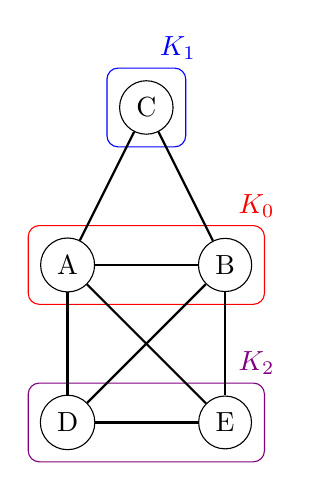
\begin{tikzpicture}
      \tikzstyle{vertex}=[draw,circle]
      \tikzstyle{edge}=[draw,thick]
      \path[draw,blue,rounded corners] (0.5,3.5) rectangle (1.5,4.5);
      \node[blue] at (1.4,4.75) {$K_1$};
      \path[draw,red,rounded corners] (-0.5,1.5) rectangle (2.5,2.5);
      \node[red] at (2.4,2.75) {$K_0$};
      \path[draw,violet,rounded corners] (-0.5,-0.5) rectangle (2.5,0.5);
      \node[violet] at (2.4,0.75) {$K_2$};
      \node[vertex] (A) at (0,2) {A};
      \node[vertex] (B) at (2,2) {B};
      \node[vertex] (C) at (1,4) {C};
      \node[vertex] (D) at (0,0) {D};
      \node[vertex] (E) at (2,0) {E};
      \path[edge] (A) -- (B);
      \path[edge] (A) -- (C);
      \path[edge] (A) -- (D);
      \path[edge] (A) -- (E);
      \path[edge] (B) -- (C);
      \path[edge] (B) -- (D);
      \path[edge] (B) -- (E);
      \path[edge] (D) -- (E);
    \end{tikzpicture}
    \caption{(a)}
  \end{minipage}
  \begin{minipage}[t]{0.31\textwidth}
    \centering
    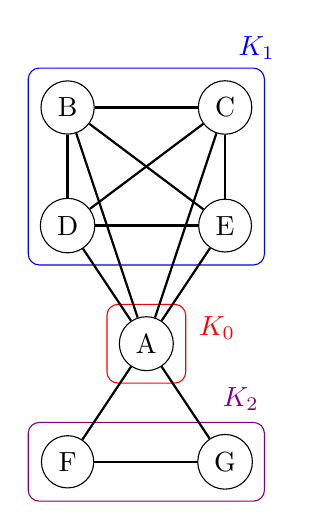
\begin{tikzpicture}
      \tikzstyle{vertex}=[draw,circle]
      \tikzstyle{edge}=[draw,thick]
      \path[draw,blue,rounded corners] (-0.5,2.5) rectangle (2.5,5);
      \node[blue] at (2.4,5.25) {$K_1$};
      \path[draw,red,rounded corners] (0.5,1) rectangle (1.5,2);
      \node[red] at (1.9,1.7) {$K_0$};
      \path[draw,violet,rounded corners] (-0.5,-0.5) rectangle (2.5,0.5);
      \node[violet] at (2.2,0.8) {$K_2$};
      \node[vertex] (A) at (1,1.5) {A};
      \node[vertex] (B) at (0,4.5) {B};
      \node[vertex] (C) at (2,4.5) {C};
      \node[vertex] (D) at (0,3) {D};
      \node[vertex] (E) at (2,3) {E};
      \node[vertex] (F) at (0,0) {F};
      \node[vertex] (G) at (2,0) {G};
      \path[edge] (A) -- (B);
      \path[edge] (A) -- (C);
      \path[edge] (A) -- (D);
      \path[edge] (A) -- (E);
      \path[edge] (A) -- (F);
      \path[edge] (A) -- (G);
      \path[edge] (B) -- (C);
      \path[edge] (B) -- (D);
      \path[edge] (B) -- (E);
      \path[edge] (C) -- (D);
      \path[edge] (C) -- (E);
      \path[edge] (D) -- (E);
      \path[edge] (F) -- (G);
    \end{tikzpicture}
    \caption{(b)}
  \end{minipage}
  \begin{minipage}[t]{0.31\textwidth}
    \centering
    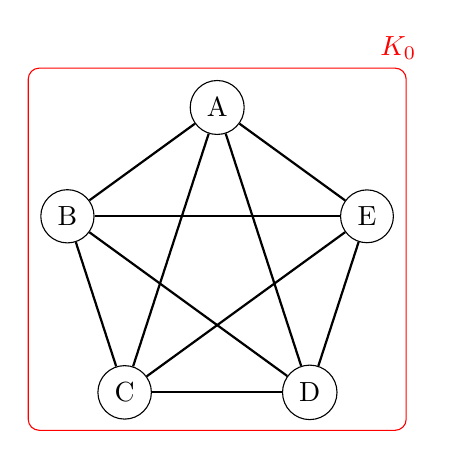
\begin{tikzpicture}
      \path[draw,red,rounded corners] (-2.4,-2.1) rectangle (2.4,2.5);
      \node[red] at (2.3,2.75) {$K_0$};
      \foreach \i / \angle / \label in {1/90/A, 2/162/B, 3/234/C, 4/306/D, 5/18/E} {
        \node[draw,circle] (\i) at (\angle:2) {\label};
      }
      \foreach \i in {1,...,5} {
        \foreach \j in {1,...,5} {
          \ifnum\i<\j
            \path[draw,thick] (\i) -- (\j);
          \fi
        }
      }
    \end{tikzpicture}
    \caption{(c)}
  \end{minipage}
\end{figure}

而到了節目後期,Ray需要舉辦一場比賽,讓所有有建立關係的任兩位參賽者都進行一次對決,並且這些對決一定會有一方獲勝。如果參賽者
\(x\)、\(y\) 進行對決並且 \(x\) 贏得勝利,則我們稱 \(x\) 比 \(y\)
強;如果參賽者 \(x\) 比 \(y\) 強並且 \(y\) 比 \(z\) 強,則我們又稱 \(x\)
比 \(z\) 強。

為了能夠決定出最終贏家(可能有多個),Ray\textbf{不希望存在三位參賽者
\(x\)、\(y\)、\(z\) 使得 \(x\) 比 \(y\) 強,\(y\) 比 \(z\) 強,但 \(z\)
又比 \(x\) 強}。

\newpage

所以他需要先私下列出一份完整勝負關係,讓所有參賽者照著這份勝負關係進行對決,使得最終結果滿足他的要求。一份勝負關係若要被稱為完整勝負關係,那\textbf{對於任兩位有建立關係的參賽者,都必須在勝負關係中決定出勝方是誰}。

如果要用圖來表示勝負關係,那麼對於任兩位有建立關係的參賽者
\(x\)、\(y\),如果 \(x\)、\(y\) 有進行對決,那就讓 \(x\)、\(y\)
之間的邊指向勝方,例如 \(x\) 贏得勝利就是指向 \(x\)。

舉例來說,圖(d)就是一份符合要求的完整勝負關係,最終贏家為C和E。圖(e)中的B、E有建立關係但沒有分出勝負,所以它不是一份完整的勝負關係。而圖(f)則是因為A比C強、C比B強、但B又比A強,所以它沒辦法決定出最終贏家。

\begin{figure}[h]
  \centering
  \begin{minipage}[t]{0.31\textwidth}
    \centering
    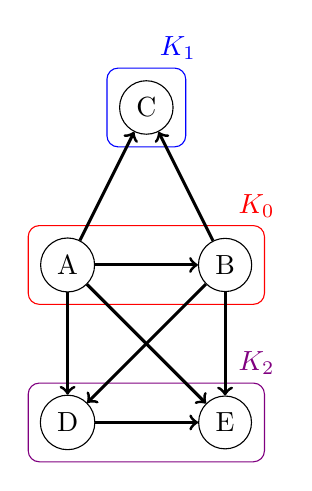
\begin{tikzpicture}
      \tikzstyle{vertex}=[draw,circle]
      \tikzstyle{edge}=[draw,line width=1.1pt,->]
      \path[draw,blue,rounded corners] (0.5,3.5) rectangle (1.5,4.5);
      \node[blue] at (1.4,4.75) {$K_1$};
      \path[draw,red,rounded corners] (-0.5,1.5) rectangle (2.5,2.5);
      \node[red] at (2.4,2.75) {$K_0$};
      \path[draw,violet,rounded corners] (-0.5,-0.5) rectangle (2.5,0.5);
      \node[violet] at (2.4,0.75) {$K_2$};
      \node[vertex] (A) at (0,2) {A};
      \node[vertex] (B) at (2,2) {B};
      \node[vertex] (C) at (1,4) {C};
      \node[vertex] (D) at (0,0) {D};
      \node[vertex] (E) at (2,0) {E};
      \path[edge] (A) -- (B);
      \path[edge] (A) -- (C);
      \path[edge] (A) -- (D);
      \path[edge] (A) -- (E);
      \path[edge] (B) -- (C);
      \path[edge] (B) -- (D);
      \path[edge] (B) -- (E);
      \path[edge] (D) -- (E);
    \end{tikzpicture}
    \caption{(d)}
  \end{minipage}
  \begin{minipage}[t]{0.31\textwidth}
    \centering
    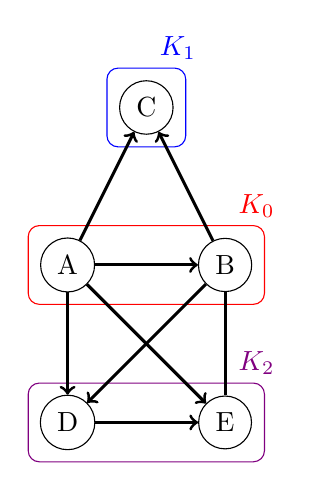
\begin{tikzpicture}
      \tikzstyle{vertex}=[draw,circle]
      \tikzstyle{edge}=[draw,line width=1.1pt,->]
      \path[draw,blue,rounded corners] (0.5,3.5) rectangle (1.5,4.5);
      \node[blue] at (1.4,4.75) {$K_1$};
      \path[draw,red,rounded corners] (-0.5,1.5) rectangle (2.5,2.5);
      \node[red] at (2.4,2.75) {$K_0$};
      \path[draw,violet,rounded corners] (-0.5,-0.5) rectangle (2.5,0.5);
      \node[violet] at (2.4,0.75) {$K_2$};
      \node[vertex] (A) at (0,2) {A};
      \node[vertex] (B) at (2,2) {B};
      \node[vertex] (C) at (1,4) {C};
      \node[vertex] (D) at (0,0) {D};
      \node[vertex] (E) at (2,0) {E};
      \path[edge] (A) -- (B);
      \path[edge] (A) -- (C);
      \path[edge] (A) -- (D);
      \path[edge] (A) -- (E);
      \path[edge] (B) -- (C);
      \path[edge] (B) -- (D);
      \path[draw,line width=1.1pt] (B) -- (E);
      \path[edge] (D) -- (E);
    \end{tikzpicture}
    \caption{(e)}
  \end{minipage}
  \begin{minipage}[t]{0.31\textwidth}
    \centering
    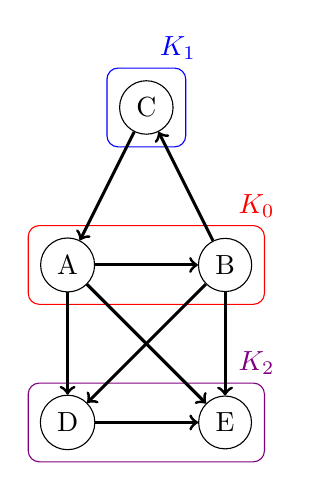
\begin{tikzpicture}
      \tikzstyle{vertex}=[draw,circle]
      \tikzstyle{edge}=[draw,line width=1.1pt,->]
      \path[draw,blue,rounded corners] (0.5,3.5) rectangle (1.5,4.5);
      \node[blue] at (1.4,4.75) {$K_1$};
      \path[draw,red,rounded corners] (-0.5,1.5) rectangle (2.5,2.5);
      \node[red] at (2.4,2.75) {$K_0$};
      \path[draw,violet,rounded corners] (-0.5,-0.5) rectangle (2.5,0.5);
      \node[violet] at (2.4,0.75) {$K_2$};
      \node[vertex] (A) at (0,2) {A};
      \node[vertex] (B) at (2,2) {B};
      \node[vertex] (C) at (1,4) {C};
      \node[vertex] (D) at (0,0) {D};
      \node[vertex] (E) at (2,0) {E};
      \path[edge] (A) -- (B);
      \path[edge] (C) -- (A);
      \path[edge] (A) -- (D);
      \path[edge] (A) -- (E);
      \path[edge] (B) -- (C);
      \path[edge] (B) -- (D);
      \path[edge] (B) -- (E);
      \path[edge] (D) -- (E);
    \end{tikzpicture}
    \caption{(f)}
  \end{minipage}
\end{figure}

Ray想要知道對於給定的超大型實境節目,總共有幾種符合要求的完整勝負關係。因為這個數字可能很大,你只要求出方法數除以
\(10^9+7\) 的餘數就行了。

\subsection{輸入格式}

\begin{format}
\f{
$t$
$n_0 \ n_1 \ n_2 \ \ldots \ n_t$
}
\end{format}

\begin{itemize}
\tightlist
\item
  \(t\) 代表小圈圈的數量。
\item
  \(n_0\) 代表屬於中心圈圈的參賽者人數。
\item
  \(n_i\) 代表屬於第 \(i\) 個小圈圈 \(K_i\)
  的參賽者人數,\(i \in \{1, 2, \ldots, t\}\)。
\end{itemize}

\subsection{輸出格式}

\begin{format}
\f{
$ans$
}
\end{format}

\begin{itemize}
\tightlist
\item
  \(ans\) 代表符合要求的完整勝負關係的數量 mod \(10^9+7\) 後的結果。
\end{itemize}

\subsection{測資限制}

\begin{itemize}
\tightlist
\item
  \(0 \leq t \leq 10^6\)。
\item
  \(1 \leq n_i \leq 10^7\)。
\item
  輸入的數皆為整數。
\end{itemize}

\subsection{範例測試}

\begin{example}
\exmp{
2
2 1 2
}{%
72
}%
\exmp{
3
5 7 6 9
}{%
6928820
}%
\end{example}

\subsection{評分說明}

本題共有四組子任務,條件限制如下所示。
每一組可有一或多筆測試資料,該組所有測試資料皆需答對才會獲得該組分數。

\begin{longtable}[]{@{}ccl@{}}
\toprule
子任務 & 分數 & 額外輸入限制 \\
\midrule
\endhead
1 & \(4\) & \(t = 0\)。 \\
2 & \(9\) & \(t \leq 1\)。 \\
3 & \(22\) & \(t \leq 2\)。 \\
4 & \(65\) & 無額外限制。 \\
\bottomrule
\end{longtable}

\section{指紋 (Fingerprint)}

\subsection{問題描述}

彼得是一個生物專家,他從不同的資料中分析同一群物種間的演化關係,經常會得到不同的演化樹,他想知道不同演化樹間的相似程度。為了節省比較時間,他的想法是先將每一棵演化樹
\(T\) 的結構用一個稱為「指紋
(fingerprint)」的數字來表示,然後再進一步去仔細比較「指紋」相近的不同演化樹。

演化樹是一棵無向無根樹 (undirected, unrooted
tree),葉節點代表現存物種。令 \(S\) 是一個現存物種集合,令 \(T\) 是
\(S\) 的一棵演化樹;也就是說 \(T\) 的葉節點集合是
\(S\);令\(\text{deg}(x)\) 表示與節點 \(x\)
相鄰之節點個數,對於一個點\(x \in T\),當\(\text{deg}(x) = 1\)時,我們稱
\(x\) 為 \(T\)
的葉節點;而不是葉節點的點就稱作為內節點,代表著物種的演化過程。對任兩個物種
\(x, y\in S\),定義它們間的距離 \(d(x, y)\) 為 \(x\) 到 \(y\) 路徑
(path) 上的邊數 (number of edges)。彼得用 \(f(T)\) 來表示 \(T\)
的「指紋」並定義 \(T\) 的「指紋」為任兩物種距離平方的總和;也就是說 \[
f(T) =  \sum_{x, y \in S, x < y} d(x, y)^2。
\] 以下圖中的演化樹 \(T\) 為例,這個演化樹的「指紋」
\(f(T) = d(1, 2)^2 + d(1, 3)^2 + d(1, 4)^2 + d(1, 5)^2 + d(2, 3)^2 + d(2, 4)^2 + d(2, 5)^2 + d(3, 4)^2 + d(3, 5)^2 + d(4, 5)^2 = 3^2 + 3^2 + 3^2 + 3^2 + 4^2 + 4^2 + 2^2 + 2^2 + 4^2 + 4^2 = 108\)。

\begin{figure}[H]
    \centering
    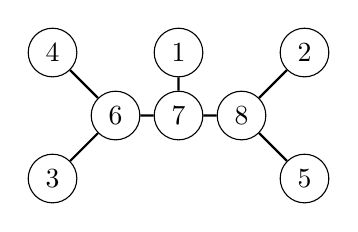
\begin{tikzpicture}[scale=0.8]
        \def \Nodes{ 1/2/2/white/black, 2/4/2/white/black, 3/0/0/white/black, 4/0/2/white/black, 5/4/0/white/black, 6/1/1/white/black, 7/2/1/white/black, 8/3/1/white/black}
        \def \Edges{ 1/7, 2/8, 3/6, 4/6, 5/8, 6/7, 7/8}
        \foreach \id / \x / \y / \c / \d in \Nodes{
            \node[draw,circle,fill=\c] (\id) at (\x, \y) {\textcolor{\d}{\id}};
        }
        \foreach \x / \y in \Edges{
            \path[draw,-,thick] (\x) -- (\y);
        }
    \end{tikzpicture}
    \caption{$圖一$}
\end{figure}

請撰寫一個程式來計算一棵演化樹 \(T\) 的「指紋」 \(f(T)\)。因為 \(f(T)\)
可能很大,所以你只要求出 \(f(T)\) 除以 \(10^9 + 7\) 的餘數。

\subsection{輸入格式}

\begin{format}
\f{
$m$
$u_1$ $v_1$
$u_2$ $v_2$
\vdots
$u_{m-1}$ $v_{m-1}$
}
\end{format}

\begin{itemize}
\tightlist
\item
  \(m\) 代表演化樹 \(T\) 的點數量。
\item
  \(u_i\) 和 \(v_i\) 代表的是在 \(T\)上 \(u_i\) 和 \(v_i\)有一條邊。
\end{itemize}

\subsection{輸出格式}

\begin{format}
\f{
$a$
}
\end{format}

\begin{itemize}
\tightlist
\item
  \(a\) 代表給定的演化樹 \(T\) 的指紋除以 \(10^9 + 7\) 的餘數。
\end{itemize}

\subsection{測資限制}

\begin{itemize}
\tightlist
\item
  \begin{math}2 \le m \le 10^6\end{math}。
\item
  \begin{math}1 \le u_i, v_i \le m\end{math}。
\item
  輸入的數皆為整數。
\item
  保證給定的圖是一棵連通的演化樹。
\end{itemize}

\subsection{範例測試}

\begin{example}
\exmp{
8
4 6
3 6
6 7
7 1
7 8
8 2
8 5
}{%
108
}%
\exmp{
2
1 2
}{%
1
}%
\end{example}

\subsection{評分說明}

本題共有三組子任務,條件限制如下所示。
每一組可有一或多筆測試資料,該組所有測試資料皆需答對才會獲得該組分數。

\begin{longtable}[]{@{}ccl@{}}
\toprule
子任務 & 分數 & 額外輸入限制 \\
\midrule
\endhead
1 & \(7\) & \begin{math}m \le 1000\end{math}。 \\
2 & \(31\) & 演化樹的所有內部節點 \(v\) 的 deg(\(v\)) 都等於
\(3\),\(m \le 10^5\)。 \\
3 & \(62\) & 無額外限制。 \\
\bottomrule
\end{longtable}

\section{海盜地圖 (Pirate)}

\subsection{問題描述}

在某個大洋中,有 \(n\) 座小島,分別編號從
\(\{1, 2, \ldots, n\}\),另外也有著 \(m\)
條航線來直接連接兩個小島。每條航線都以一組數字 \(x, y\) 表示
,代表透過這條航線從小島 \(x\) 行船至小島 \(y\)
只需要一單位的時間,反之從小島 \(y\) 行船至小島 \(x\)
也只需要一單位的時間。然而並不是任兩個小島 \(x\) 和 \(y\)
都有一條航線直接連接,這時要從 \(x\) 行船至
\(y\),需要透過一系列的小島作為中間接駁的島。具體來說,我們需要一系列的小島
\(a_1, a_2, \ldots, a_k\),其中 \(x = a_1,y = a_k\),而且對於所有
\(1 \leq i \leq k-1\),\(a_i\) 和 \(a_{i+1}\)
有航線直接相連,這會是一個間接連接小島 \(x\) 和 \(y\)
的方式,並且需要花費 \(k-1\)
單位的時間。兩個小島之間的最快速行船路線的所需時間為所有能滿足上列要求的序列所需花費時間的最小值。並且任意兩個小島都能透過這些航線直接或間接的連接。

另外在每座小島都有一組海盜佔據著,他們各自紀錄著從他們所在的小島至各個島的最快速行船路線的所需時間。由於海盜們十分忙碌,有些需要花費比較長時間的行船路線,會隨著時間的過去,而忘記確切的所需時間。只能確定這些被遺忘的最快速行船路線的所需時間的值\textbf{至少嚴格大於
\(\sqrt{n}\)。}

\begin{figure}[!htb]
  \centering
  \includegraphics[width=0.3\linewidth]{pirate.png}
  \caption{圖片來源:產生自 ChatGPT}
\end{figure}

海盜們將航線的完整資訊寄給你,並給 \(q\)
組被遺忘的路線,希望你幫他們算出這些已忘記的最快速行船路線的所需時間。

\subsection{輸入格式}

\begin{format}
\f{
$n$ $m$ $q$
$x_1$ $y_1$
$x_2$ $y_2$
$\vdots$
$x_m$ $y_m$
$s_1$ $t_1$
$s_2$ $t_2$
$\vdots$
$s_q$ $t_q$
}
\end{format}

\begin{itemize}
\tightlist
\item
  \(n\) 代表小島數。
\item
  \(m\) 代表海盜給出的航線數。
\item
  \(q\) 代表忘記所需時間的最快速行船路線數量。
\item
  \(x_i, y_i\) 代表有一條航線直接連接著小島 \(x_i\) 和 \(y_i\)。
\item
  \(s_i, t_i\) 代表海盜遺忘的第 \(i\) 條路線。
\end{itemize}

\subsection{輸出格式}

\begin{format}
\f{
$d_1$ $d_2$ $\ldots$ $d_q$
}
\end{format}

\begin{itemize}
\tightlist
\item
  \(d_i\) 代表海盜遺忘的第 \(i\) 條路線所需的最快速行船時間。
\end{itemize}

\subsection{測資限制}

\begin{itemize}
\tightlist
\item
  \(1 \leq n \leq 10^4\)。
\item
  \(1 \leq m \leq 10^5\)。
\item
  \(1 \leq q \leq 3\times 10^4\)。
\item
  \(1 \leq x_i, y_i \leq n,x_i \neq y_i\)。
\item
  \(1 \leq s_i, t_i \leq n\)。
\item
  保證所有被遺忘的路線皆滿足其最快速行船路線的所需時間的值\textbf{至少嚴格大於
  \(\sqrt{n}\)。}
\item
  海盜給出的航線都是相異的。
\item
  保證任意兩個小島都能透過這些航線直接或間接的連接。
\item
  輸入的數皆為整數。
\end{itemize}

\subsection{範例測試}

\begin{example}
\exmp{
4 3 2
1 2
2 3
3 4
1 4
4 1
}{%
3 3
}%
\end{example}

\subsection{評分說明}

本題共有四組子任務,條件限制如下所示。
每一組可有一或多筆測試資料,該組所有測試資料皆需答對才會獲得該組分數。

\begin{longtable}[]{@{}ccl@{}}
\toprule
子任務 & 分數 & 額外輸入限制 \\
\midrule
\endhead
1 & \(6\) & \(n \le 500\)。 \\
2 & \(17\) & \(n \le 5\times 10^3\),\(m \le 10^4\)。 \\
3 & \(21\) & 詳見備註(一)。 \\
4 & \(56\) & 無額外限制。 \\
\bottomrule
\end{longtable}

備註(一):存在至多 \(1000\) 個特別小島,使得所有被遺忘的從小島 \(x\)
至小島 \(y\) 最快速行船路線的所需時間,不是 \(x\) 是特別小島,就是 \(y\)
是特別小島。
